\chapter{Methodology} \label{Chap3}

\section{Theorem behind the Search Algorithm}

\subsection{Producing All Logical Cliffords}
The underlying theorem behind the search algorithm was found by my supervisor Dr. Mark Webster (paper under development). The theorem can be described as follows:

\begin{theorem}
    Let \(\tau\) be the symplectic matrix (tableau) of the encoding operator of an \([[n,k]]\) stabiliser code and let $U$ be a Clifford unitary on \(k\) qubits. The logical Clifford operators with action \(U\) are of the form:
    \begin{equation}
    \label{eq:Generation of Logical operator}
        \bar{U}:=\tau^{-1}\left(\left( I\otimes U\right)U_C U_A\right)\tau
    \end{equation}
    where \(U_A, U_C\) have symplectic representations of the following form:
    \begin{equation}
        U_A := \left[\begin{array}{cc|cc}I&0&0&0\\0&I&0&0\\\hline A_1&A_2^T&I&0\\A_2&0&0&I\end{array}\right]
    \end{equation}
    \begin{equation}
        U_C := \left[\begin{array}{cc|cc}C_1&0&0&0\\C_2&I&0&0\\\hline 0&0&C_1^{-T}&C_1^{-T}C_2^T\\0&0&0&I\end{array}\right]
    \end{equation}
    
    Note that symplectic matrices act on Paulis by right matrix multiplication, so order of operations is reversed. In the above forms, \(r:=n-k\),  \(A_1\) is a symmetric \(r\times r\) matrix, \(C_1\) is an invertible \(r\times r\) matrix, \(A_2,C_2\) are arbitrary \(k\times r\) matrices and  \(C_1^{-T} := \left(C_1^{-1}\right)^T\).
\end{theorem}

This theorem states that given a unitary Clifford operator, \(U\), and the encoding operator, \(\tau\),  we can create all Logical Cliffords, \(\bar{U}\), with the desired action \(U\), by considering all possible forms of \(U_A\) and \(U_C\). The figure below provides an intuitive visualisation of Equation \ref{eq:Generation of Logical operator}.We can interpret the logical operation \(\bar{U}\) as a three-step process: first, the encoded quantum state is decoded by applying the inverse of the encoding operation, \(\tau^{-1}\), then, the desired single-qubit Clifford operation \(U\) is applied to the logical subspace; and finally, the state is re-encoded using \(\tau\), mapping it back into the protected code space. This sequence effectively implements the logical Clifford \(\bar{U}\) on the encoded state by conjugating the logical action through the encoding circuit.

\begin{figure}[h]
    \centering
    \begin{large}
    \begin{tikzcd}
    \mathcal{H}_2^{n-k} \otimes \mathcal{H}_2^k \arrow[r, "\mathcal{\tau}"] \arrow[d, " (I \otimes U)\, U_C\, U_A"'] &
    \mathcal{H}_2^n \arrow[d, "\overline{U}"] \\
    \mathcal{H}_2^{n-k} \otimes \mathcal{H}_2^k \arrow[r, "\mathcal{\tau}"] &
    \mathcal{H}_2^n
    \end{tikzcd}
    \end{large}
    \caption{Hilbert space diagram for generating all logical Cliffords}
    \label{fig:Hilbert space diagram}
\end{figure}

An important corollary in the synthesis of logical Clifford operators is the count of distinct Clifford operators that implement a given logical action \(U\), up to signs and stabiliser equivalence (i.e., modulo Pauli operators). The total number of such implementations, \(N\), is given by,

\begin{equation}
\label{eq:number of possible logical cliffords}
   N=2^{2rk + r(r+1)/2}\prod_{0 \le i \le r-1}(2^r - 2^i)
\end{equation}

where \(r=n-k\) is the number of stabiliser generators. This expression arises from the number of valid choices for the matrices \(A_1,A_2,C_1,\) and \(C_2\) that define different Clifford encodings with the same logical effect. Specifically, \(A_1\) is any symmetric \(r\times r\) binary matrix, contributing \(2^{r(r+1)/2}\) possibilities, \(A_2\) and \(C_2\) are arbitrary \(r\times k\) binary matrices, each contributing \(2^{rk}\), and \(C_1\) is any invertible \(r\times r\) binary matrix, with \(\prod_{0 \le i \le r-1}(2^r - 2^i)\) valid choices. The resulting product accounts for the total number of distinct tableau encodings realising the same logical Clifford. 

Given the exponential number of possible logical Clifford implementations described by Equation \ref{eq:number of possible logical cliffords}, an exhaustive search over all valid combinations of \(A_1,A_2,C_1,\) and \(C_2\) becomes computationally infeasible for even modest values of \(n\) and \(k\) To overcome this, we have developed a search algorithm that leverages metaheuristic techniques to efficiently explore the vast solution space and identify logical Clifford implementations that minimise the number of two-qubit transvections. By focusing on solutions with the lowest entangling gate count, the algorithm finds not only optimal decompositions using two-qubit transvections, SWAPs, and single-qubit Clifford gates, but also does so with significantly reduced computational overhead compared to brute-force methods. The exponential reduction in time provided by using metaheuristic techniques is particularly valuable as there exist hundreds of stabiliser codes, each requiring its own distinct set of logical operators. The impracticality of brute-force synthesis across all codes makes scalable, optimised search strategies a crucial step toward practical fault-tolerant quantum circuit design.

\subsection{Decomposition of Logical Cliffords into SWAPs, 2-Qubit Transvections and Single-Qubit Cliffords}

In this section, we briefly mention the method used to decompose logical Clifford operators. The decomposition approach was developed by Kalle Volanto in his thesis Minimising the Number of Two-qubit Gates in Clifford Circuits \cite{volanto2023minimizing}, where a complete and detailed description of the method can be found. My supervisor, Mark, has implemented this decomposition in Python, allowing us to apply it directly to logical Cliffords. This is particularly important for our purposes, as it enables us to score the logical Cliffords based on the number of two-qubit transvections required. (see Appendix \ref{Appendix B} for more details)

\section{Algorithm Design}

\subsection{Overview of the Framework}
Given that we can decompose logical Cliffords into SWAPs,  2-Qubit Transvections and Single-Qubit Cliffords. The central goal of the algorithm is to identify the matrices \(U_A\) and \(U_C\) that construct a logical Clifford operator corresponding to a desired logical action, while minimising the number of two-qubit transvections required in its decomposition. This is achieved by exploiting the structure provided by the logical Clifford generation theorem (see Equation \ref{eq:Generation of Logical operator}), which allows all valid logical implementations to be expressed in terms of a parameterised family of symplectic matrices determined by the binary matrices 
\(A_1,A_2,C_1,\) and \(C_2\) .

The algorithm adopts a metaheuristic search strategy, inspired by evolutionary algorithms \cite{luke2009essentials}. It operates over a large, high-dimensional discrete space defined by candidate encodings of the matrices 
\(U_A\) and \(U_C\), which jointly determine the operator \((I \otimes U)\, U_C\, U_A\) in the logical construction. The algorithm begins by generating a large, random initial population of candidate \((U_C,U_A)\) pairs from the \(GL_2\) group. Each candidate is evaluated using a cost function that returns a score vector, where each entry corresponds to the number of two-qubit transvections involving a particular qubit, rather than a single total count. This scoring approach is advantageous because optimal decompositions tend to exhibit a more balanced distribution of transvections across qubits, as opposed to concentrating entangling operations on a small subset. In addition to this, finding solutions with a larger distribution of transvections across qubits are beneficial as concentrating two-qubit transvections on a limited subset of qubits can lead to increased local error rates and potential circuit bottlenecks.

A generational process is then used to iteratively refine the population. In each generation, a mixture of elitism (retaining the best performing candidates) and tournament selection (probabilistic selection based on performance) is used to choose individuals for reproduction. These selected candidates are mutated to introduce variation in the population, promoting exploration of the solution space. Two types of mutation operations are employed. The first involves performing row operations on the matrix \(C_1\), specifically adding one row to another modulo 2. This operation is well-suited to the structure of \(C_1\), as it preserves its invertibility, a necessary condition since \(C_1\) must remain an invertible \(r\times r\) matrix, and allows the algorithm to traverse the full space of invertible binary matrices \cite{gregor2024generatinginvertiblematricesrow}. The second type of mutation consists of applying arbitrary bit-flips to entries in a combined matrix containing \(A\) and \(C_2\). This is justified by the fact that both \(A_2\) and \(C_2\) are unconstrained binary matrices and can therefore be freely modified without violating structural requirements. For the symmetric matrix \(A_1\), its symmetry is maintained by restricting bit-flips to one side of the diagonal and reflecting the change across the diagonal, ensuring the matrix remains symmetric post-mutation.

These carefully designed mutations enable the algorithm to explore a broad and valid subset of the solution space efficiently, while ensuring that all algebraic constraints of the decomposition framework are respected. After mutation, the new population is re-evaluated, and the optimisation loop continues over multiple generations, gradually converging toward decompositions that minimise the number of two-qubit transvections.

Incorporating an adaptive mutation mechanism into the algorithm is crucial for addressing stagnation, which often arises when the search process becomes trapped in local minima. By detecting when improvements plateau, the algorithm can dynamically increase mutation strength, thereby enhancing exploration capabilities to escape these local optima and continue progressing toward high-quality solutions. This balance between exploration and exploitation is fundamental in evolutionary algorithms to maintain search efficacy across complex fitness landscapes.

To further enhance the robustness and search coverage of the algorithm, multiple independent populations are run in parallel. In our case we were able to simulate a maximum of 8 populations in parallel using multi-pool processing. Each process executes its own instance of the optimisation loop with a different random seed. This simple parallelisation strategy helps simulate a multi-start search without inter-process communication, improving the likelihood of finding globally optimal or near-optimal decompositions. This approach not only accelerates the discovery of promising regions in the search space but also reduces the risk of all search paths converging prematurely on local minima. Much like adaptive mutation, parallel independent populations provide an effective mechanism for diversifying the search trajectory, helping to ensure that global or near-global solutions are more likely to be found.

By combining efficient candidate generation, transvection-aware cost evaluation, and robust search dynamics, this framework provides a scalable and effective method for synthesising low-depth logical Clifford operators tailored to a given stabiliser code. The full procedure is outlined in Algorithm~\ref{alg:logical_clifford_construction}, which summarises the key steps of the search and optimisation process, from population initialisation through mutation, evaluation, and convergence. 

The pseudo code for the Algorithm is provided below. (See Appendix \ref{Appendix A} for sorce code)

\begin{algorithm}[H]
\caption{Algorithm for Optimal Logical Clifford Construction}
\label{alg:logical_clifford_construction}
\begin{algorithmic}[1]
\Require Encoding tableau \(\tau\), target Clifford \(U\)
\Ensure Optimal logical Clifford implementation \(\bar{U}\)
\State Compute inverse tableau \(\tau^{-1}\), set \(n, k, r = n-k\)
\State Initialise parameters, e.g population sise, number generations, ..., etc
\Statex
\State Randomly generate initial population of \((U_C, U_A)\) candidates
\State Create \(\bar{U}\) from Equation \ref{eq:Generation of Logical operator} using \(U,(U_A,U_C),\tau\), and \(\tau^{-1}\)
\State Decompose \(\bar{U}\) into 2-qubit transvections, SWAPS, and single qubit Cliffords 
\State Evaluate initial scores based on gate count on each qubit 
\State Store best candidate and score
\Statex
\For{each generation \(g\)}
    \State Select the top x (\(U_C,U_C\)) candidates by score (elite group)
    \State Select y others using tournament selection
    \Statex \hspace{1.5em} \(\rightarrow \) Randomly partition population into \(y\) groups (tournaments)
    \Statex \hspace{1.5em} \(\rightarrow \) In each group, evaluate scores of candidates
    \Statex \hspace{1.5em} \(\rightarrow \) Select the best-performing candidate from each group (winner)
    \State Combine elite group and tournament winners
    \Statex
    \State Mutate each candidate \(\lambda\) times to generate next generation
    \Statex
    \State Evaluate new population scores using steps 4-6
    \Statex
    \If{any candidate improves the best score}
        \State Update best score and reset stagnation counters
    \Else
        \State Increment stall and fertility counters
    \EndIf
    \If{stagnation exceeds threshold}
        \State Increase mutation strength to escape local minima
    \EndIf
    \If{transvection count = 0 (perfect solution found)}
        \State \textbf{break}
    \EndIf
\EndFor
\State \Return best score, best candidate
\end{algorithmic}
\end{algorithm}

\subsection{Parameter Selection and Tuning}
The performance and effectiveness of the algorithm are heavily influenced by the choice of several key parameters, including population size, number of mutations, mutation strength, elite fraction, tournament size, and the number of generations. Careful tuning of these parameters is essential to strike the right balance between exploration and exploitation, maximise convergence speed, and ensure that high-quality solutions are reliably found. To guide this selection process, a combination of empirical experimentation and theoretical intuition was employed.

Parameter tuning was carried out through a series of controlled small-scale tests on the \([[5,1,3]]\) and \([[7,1,3]]\) stabiliser codes to find zero 2-qubit transvection implementations of Logical \(H\), both of which have well-understood, constant-depth logical Clifford decompositions. For these codes we define the algorithms success by wether or not it is able to find an implementation of the logical Clifford with zero 2-qubit transvections. (Note: the success rate is for an individual population as opposed to looking at multiple populations in parallel). These benchmark codes provided a reliable foundation for evaluating algorithm performance. To ensure consistency and isolate the effect of individual parameters, each test was conducted using a fixed set of control parameters: a tournament size of 8, an elite fraction of 0.3, and no adaptive mutation. These values served as a baseline against which the impact of parameter variations could be measured.

Given the stochastic nature of metaheuristic algorithms, a fixed global random seed was used across all runs to ensure reproducibility and enable direct comparisons between different configurations under identical initial conditions. Success was defined as achieving a score of zero, meaning that the resulting logical Clifford decomposition required no two-qubit transvections, the most expensive operations in terms of error rate and circuit depth. In the following subsections, we examine the parameters to which the algorithm is most sensitive, supported by both experimental data and theoretical insights.

The first parameter we examine is the tournament size. Selecting an appropriate tournament size is especially important when considering how the algorithm should scale for larger stabiliser codes. We found that a reliable way to scale tournament size is by first considering the number of offspring each individual produces, denoted by \(\lambda\). The value of \(\lambda\) is designed to scale with the number of possible mutations an individual can undergo. As the code size increases, the mutation space grows rapidly, almost exponentially in practice. For instance, the \([[5,1,3]]\) code has 36 possible mutations, while the \([[7,1,3]]\) and \([[9,1,3]]\) codes have 78 and 136, respectively.

To maintain a healthy balance between exploitative (intensifying search around good solutions) and explorative (diversifying the search space) behaviour, we define \(\lambda\) as a fraction of the total number of mutation possibilities, specifically \((total\space possible\space mutations)/(n-1)\), which scales naturally with the number of qubits \(n\). Once \(\lambda\) is set, the tournament size can then be chosen to scale accordingly, ensuring that selection pressure remains balanced as the code scales. This adaptive approach helps maintain consistent algorithmic performance across a wide range of code sizes.

\begin{figure}[h]
    \centering
    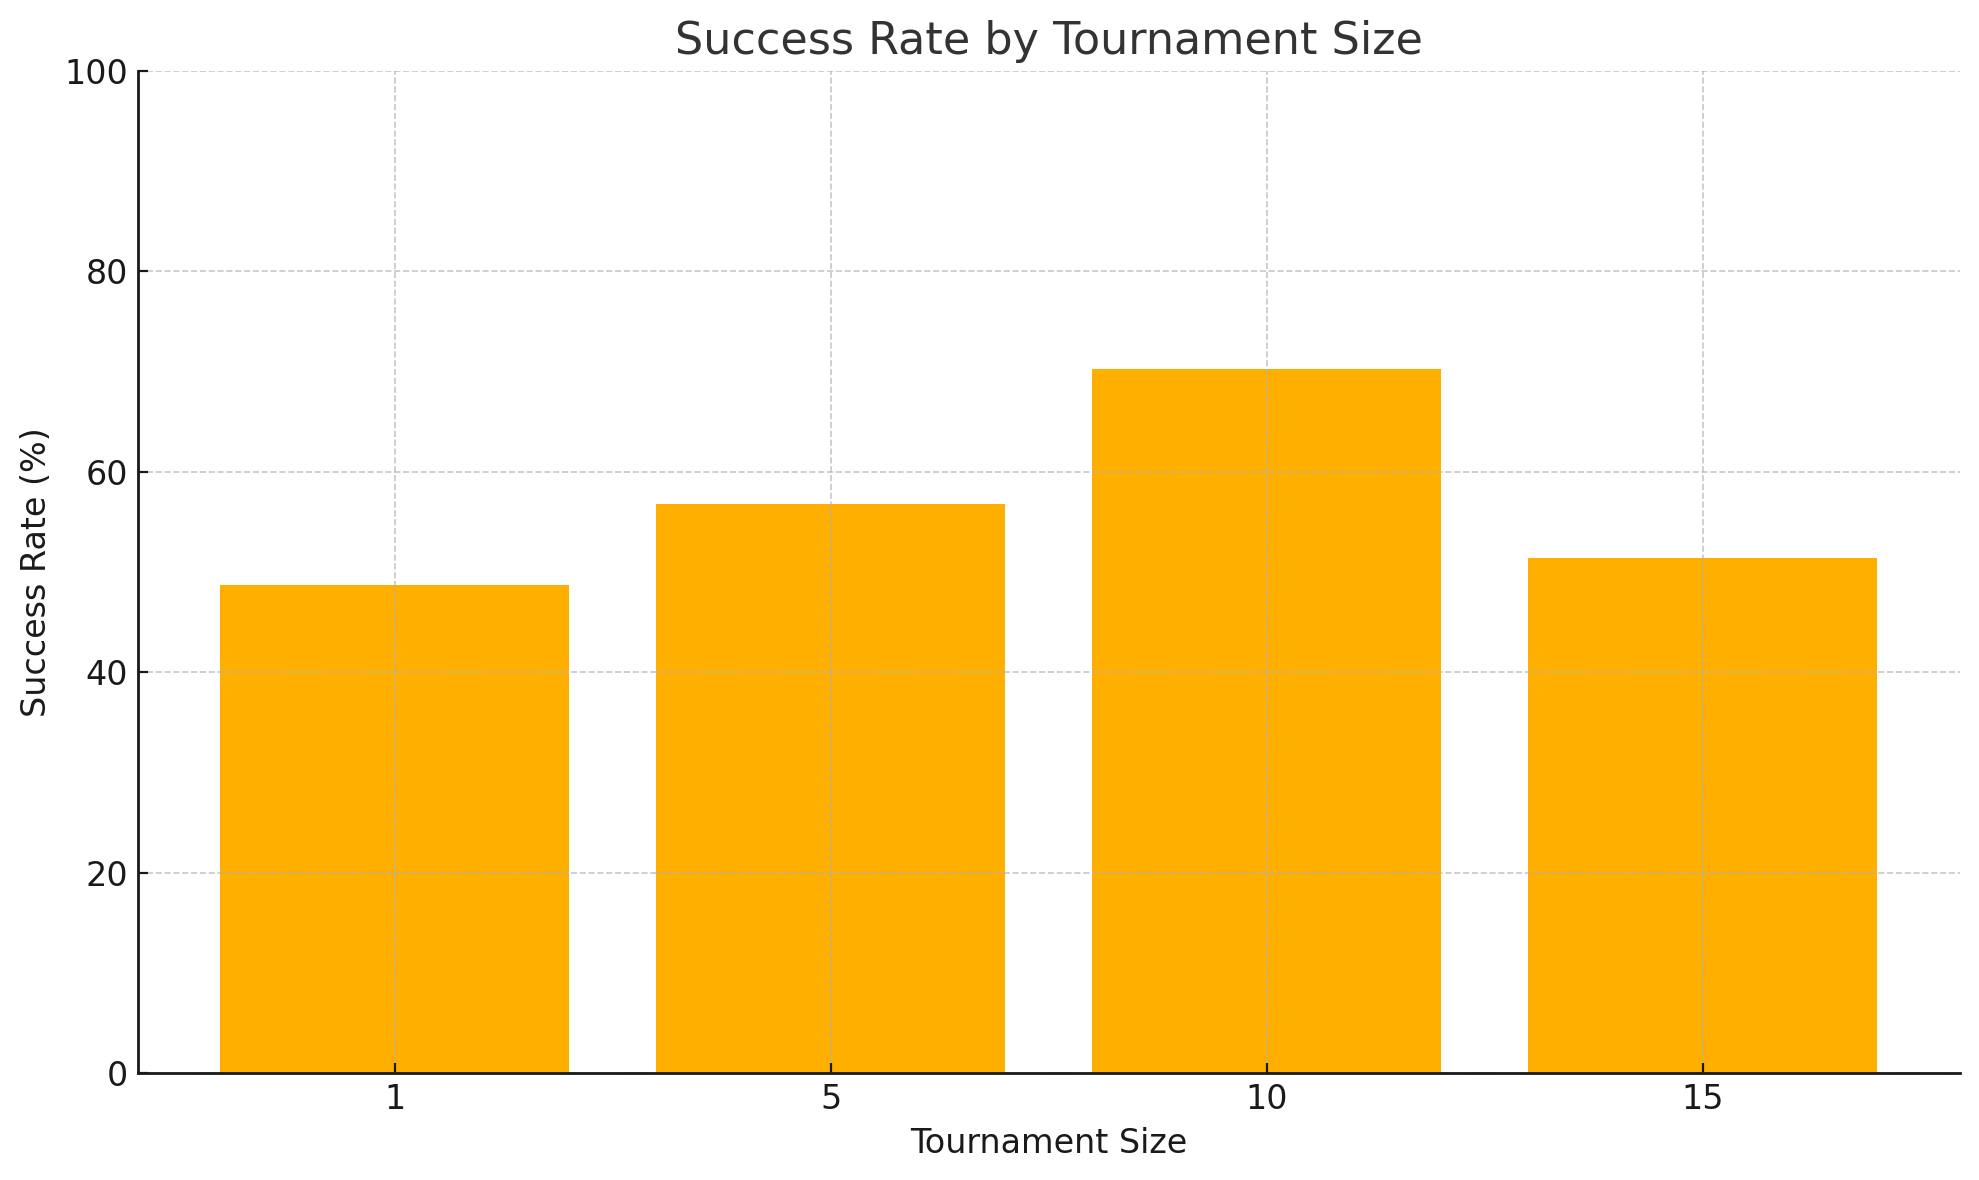
\includegraphics[width=1\linewidth]{Logos/output-2.png}
    \caption{Logical \(H\) Success rate on [[5,1,3]] code against tournament size. Number of runs = 38, elite fraction = 0.3.}
    \label{fig: tournament size chart}
\end{figure}

As shown in Figure \ref{fig: tournament size chart}, a tournament size of 10 yields the highest success rate of \(70.3\%\). This value coincides with a 1:1 ratio between \(\lambda\) and the tournament size, supporting the intuition that matching selection pressure to mutation scope leads to more effective search dynamics. Tournament sizes smaller than \(\lambda\) tend to reduce selection pressure, allowing weaker candidates to propagate and potentially slowing convergence. Conversely, larger tournament sizes increase selection pressure too aggressively, risking premature convergence to suboptimal solutions. These results affirm that scaling tournament size in proportion to \(\lambda\) provides a consistent and effective selection mechanism.

Another parameter to which the algorithm's success rate showed strong sensitivity is the elite fraction, which controls the proportion of candidates preserved from the previous generation through elitism. In this context, elites are defined as the individuals with the lowest number of two-qubit transvections, as measured by their score vectors. Adjusting the elite fraction directly influences the balance between exploitation, refining high-performing regions of the search space, and exploration, encouraging diversity and avoiding premature convergence.

A higher elite fraction places greater emphasis on preserving top candidates, which can accelerate convergence but also risks trapping the algorithm in local minima due to reduced variation. On the other hand, a lower elite fraction introduces more stochasticity through mechanisms like tournament selection, helping the algorithm explore new regions of the search space at the cost of slower convergence. 

\begin{figure}[h]
    \centering
    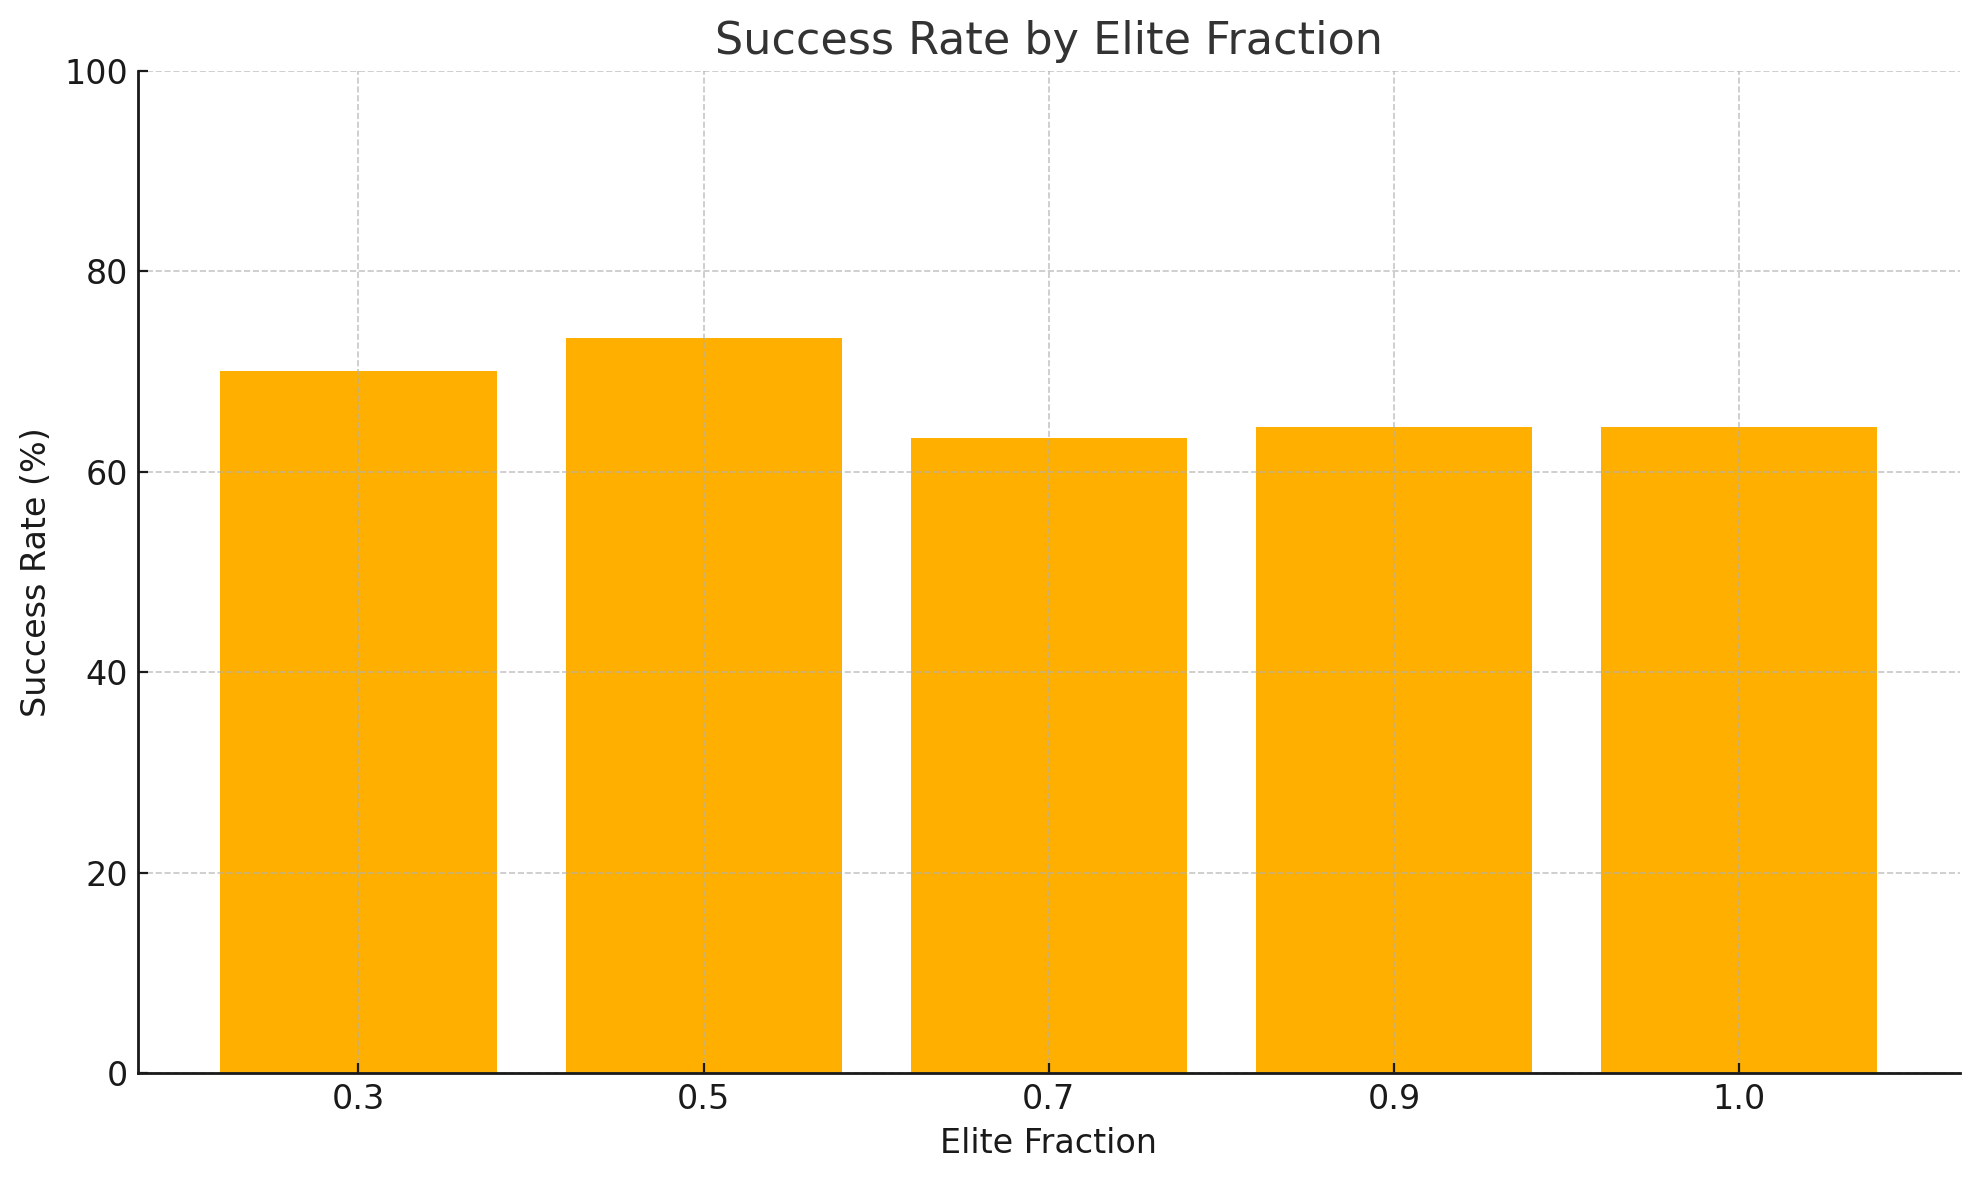
\includegraphics[width=1\linewidth]{Logos/output-3.png}
    \caption{Logical \(H\) Success rate on [[5,1,3]] code against elite fraction. Number of runs = 90, tournament size=8.}
    \label{fig: Elite fraction chart}
\end{figure}

As shown in Figure~\ref{fig: Elite fraction chart}, the highest success rate is achieved with an elite fraction of 0.5, reaching \(73.3\%\). This result supports the intuition that a balanced elitism strategy is most effective, preserving enough high-quality candidates to drive convergence, while still allowing sufficient diversity for the algorithm to escape local optima and generalise across different problem instances.

The final parameter we examine is the adaptive mutation mechanism, which plays a critical role in helping the algorithm escape local minima during the optimisation process. Several factors influence its design and effectiveness, including when to activate stronger mutations, how intense those mutations should be, and how frequently they are allowed to occur.

Our implementation uses a binary adaptive mutation strategy, alternating between two levels of mutation intensity: a fine-tuning mutation, where a single row operation or bit-flip is applied, and a strong mutation, where multiple such operations are performed on a single offspring. The central idea is that, when the population's performance stagnates, i.e., when no improvement is observed in the best candidate for several consecutive generations, it likely indicates that the search has become trapped in a local minimum. In these cases, strong mutation is temporarily activated to introduce more disruptive variation into the population, helping it escape the local basin of attraction and explore new regions of the search space.

\begin{figure}[h]
    \centering
    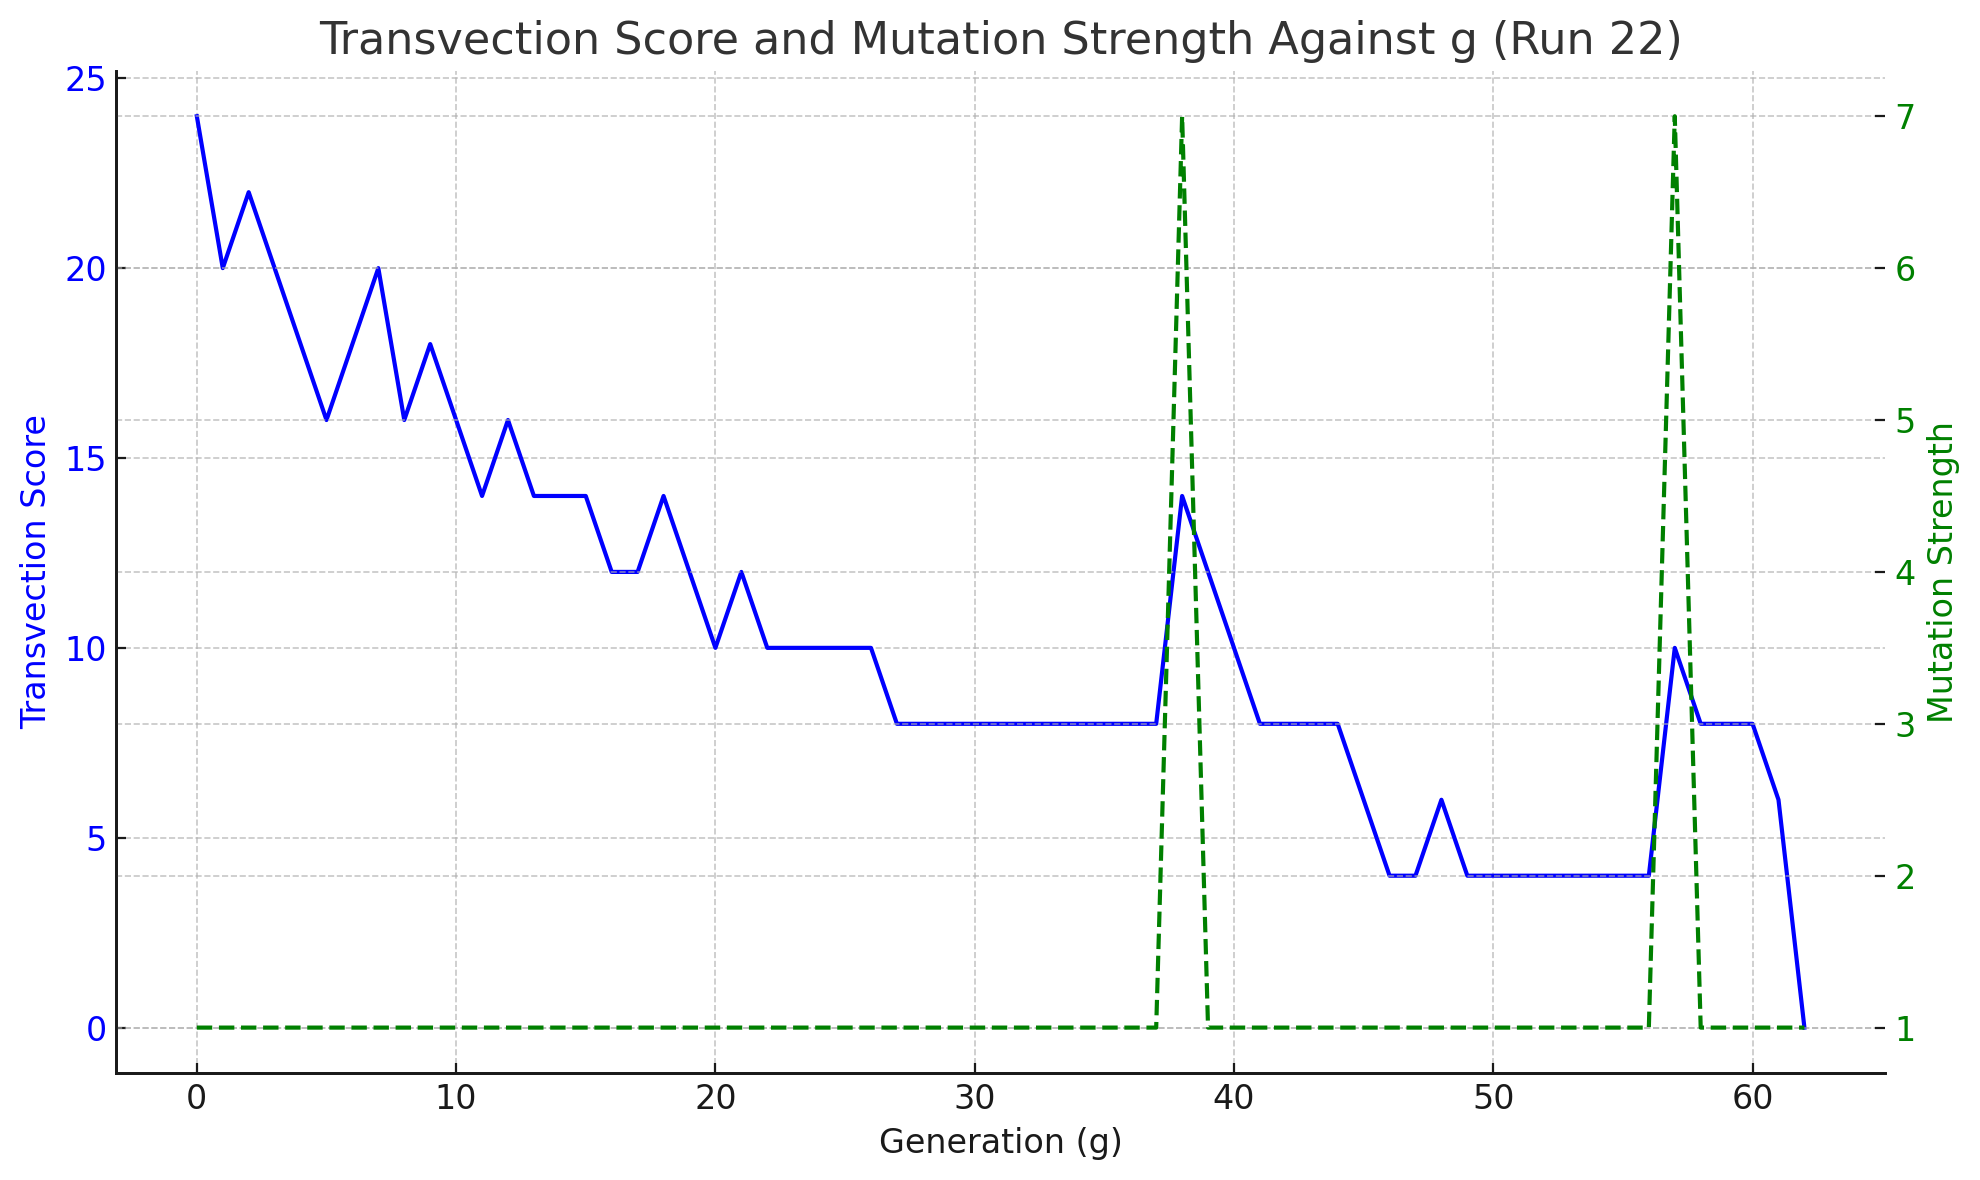
\includegraphics[width=1\linewidth]{Logos/output-4.png}
    \caption{Plot showing the total number of transvections per generation overlapped with the mutation strength across each generation on a single run of the [[7,1,3]] code to find lofical \(H\).}
    \label{fig: Adaptive Mutation tracker}
\end{figure}

Through empirical testing on the \([[5,1,3]]\) and \([[7,1,3]]\) codes, we found that strong mutation scales naturally with the number of qubits \(n\). Specifically, setting the strong mutation strength equal to \(n\) (i.e., 5 and 7 mutations respectively for the 5- and 7-qubit codes) yielded consistently good performance. In Figure \ref{fig: Adaptive Mutation tracker} we see how the transvection score evolves over generations alongside changes in mutation strength. The blue line represents the transvection score, which generally decreases as the algorithm progresses, indicating improved solutions. The green dashed line tracks the mutation strength, which increases adaptively when the score plateaus, signalling stagnation in the search process. Notably, spikes in mutation strength occur around generations 38 and 57, triggering a subsequent drop in transvection score shortly after. This illustrates the effectiveness of the adaptive mutation mechanism in helping the algorithm escape local minima and resume meaningful progress.

The experiments provided above, along with many more fine-tuning experiments, significantly contributed to the final model used to obtain the results, ensuring that the algorithm is well-calibrated for discovering low-transvection logical Clifford implementations across a range of stabiliser codes. These tests not only validated the effectiveness of individual parameter choices but also demonstrated their interplay in achieving robust, high-performance optimisation. The resulting configuration strikes a practical balance between search efficiency, solution quality, and scalability, making it suitable for use on a broad class of codes with varying sizes and structural properties.

\section{Rejected Approaches and Design Trade-offs}

\subsection{Evolutionary vs Greedy}
In this section, we briefly discuss alternative algorithmic approaches that were explored during development but ultimately deemed unsuitable for this task. While the backbone of the final implementation is an evolutionary search algorithm, one alternative we investigated was a greedy search strategy. In this approach, rather than sampling a fraction of possible single mutations per individual (as done in the evolutionary method), the algorithm exhaustively evaluates all possible single mutations and selects the best one at each step, proceeding iteratively in this greedy manner.

This method demonstrated promising results on smaller codes, such as the \([[5,1,3]]\) stabiliser code, especially when combined with enhancements like simulated annealing to introduce some stochasticity. In those cases, success rates were comparable to those achieved by the evolutionary algorithm. However, the greedy approach came with several significant drawbacks.

\begin{figure}[h]
    \centering
    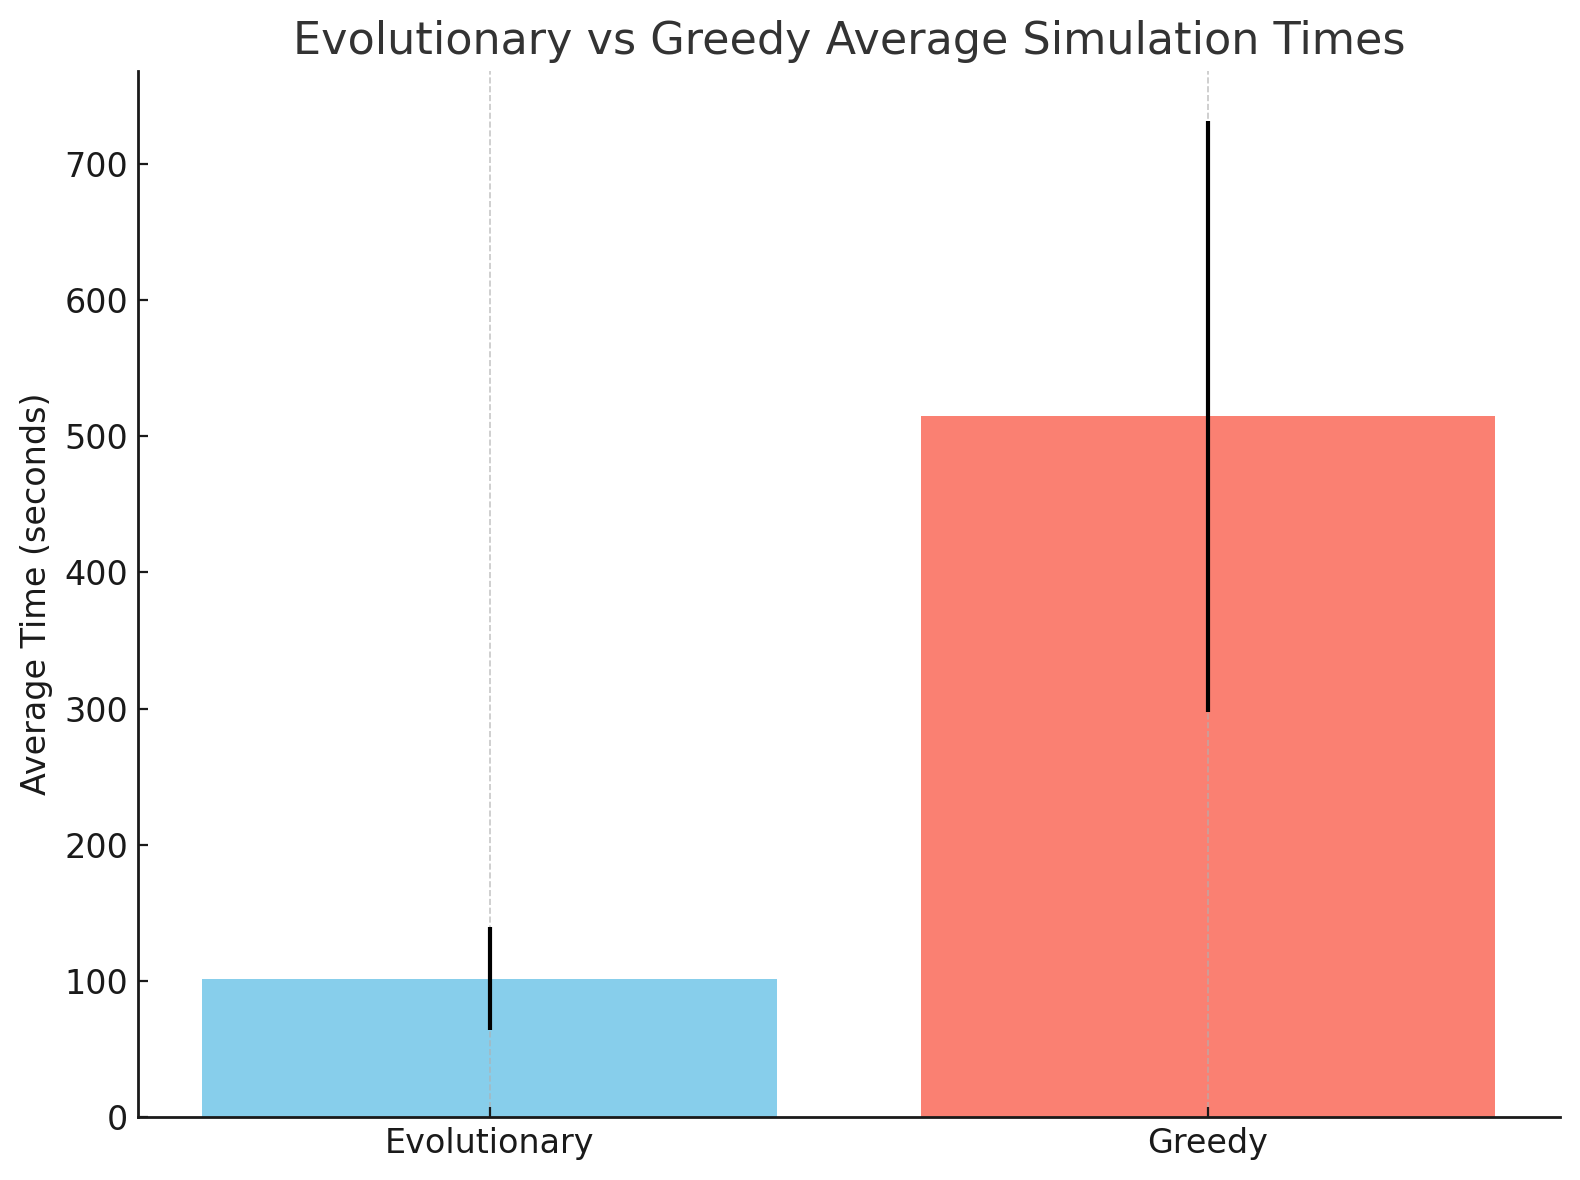
\includegraphics[width=1\linewidth]{Logos/output-5.png}
    \caption{Average simulation times on the \([[5,1,3]]\) code to find logical \(H\) for a standard Evolution and standard Greedy search algorithm. Number of runs = 36.}
    \label{fig:Evo vs Greedy simulation times}
\end{figure}

The most significant issue encountered was computational cost. Figure \ref{fig:Evo vs Greedy simulation times} compares the average execution times of the standard evolutionary algorithm and the greedy search algorithm. It is evident that the greedy approach is considerably slower, with an average runtime of \(515\) seconds per run, compared to just \(102\) seconds for the evolutionary algorithm. This discrepancy arises from the fundamental difference in how the two algorithms explore the mutation space. The evolutionary algorithm evaluates only a fraction, specifically \(1/(n-1)\), of the total mutation space per generation, the greedy approach examines the full set. This leads to an approximate runtime increase by a factor of \(n-1\), which becomes particularly prohibitive as the number of qubits grows. Moreover, the greedy method exhibited poor scalability. For larger codes, the mutation space becomes more rugged and populated with local minima, and the greedy approach by its very nature, lacks the exploration capabilities necessary to escape such traps. As a result, it often became stuck in suboptimal regions of the search space.

These limitations, both in terms of efficiency and robustness, ultimately led us to favour the evolutionary strategy, which strikes a more effective balance between exploration and exploitation and scales more gracefully with increasing code complexity.

\subsection{Dynamic Parameters}
Parameters such as the elite fraction, tournament size, and binary adaptive mutation strength were also considered in dynamic forms, meaning they would vary across generations during a single run, rather than remaining fixed. The motivation behind this approach was to better align the algorithm's behaviour with the demands of different phases of the search: for instance, using more exploration in early stages and gradually shifting toward exploitation in later ones.

However, our initial experiments with dynamic parameter schedules, conducted on the \([[5,1,3]]\) and \([[7,1,3]]\) codes, revealed mixed results. In most cases, the success rate either matched or fell slightly below that of the static configuration used in the final model. This may be partially attributed to the limited scope of codes tested; with only two small codes considered, it is difficult to draw definitive conclusions about the broader potential of dynamic parameters across more complex scenarios.

Another factor that may have influenced the outcome is the lack of optimisation in how the parameters changed over time for example, the rate at which elite fraction or mutation strength increased or decreased may not have been well-suited to the landscape of the optimisation problem. Without a principled or adaptive schedule, dynamic tuning can introduce instability or prevent the algorithm from settling into a productive search regime.

That said, this line of investigation remains promising, particularly for larger codes where the search dynamics may benefit more from stage-dependent behaviour. Future work could explore more data-driven or feedback-based scheduling of dynamic parameters, possibly leveraging online performance indicators such as population diversity or convergence rate to guide the adjustment process. 